\documentclass[a4paper, 11pt]{article}

\voffset -0cm
\hoffset 0.0cm
\textheight 23cm
\textwidth 16cm
\topmargin 0.0cm
\oddsidemargin 0.0cm
\evensidemargin 0.0cm

\usepackage{epsfig}  
\usepackage{setspace}
\usepackage{fancyheadings}
\usepackage{amsmath}
\usepackage{amssymb}
\usepackage{graphicx}
\usepackage{url}

\title{}
\author{}
\date{}

\newtheorem{qu}{Question}

\begin{document}

\begin{center}
	\LARGE \textbf{Project: ``Differential estimators distance transformation''}
\end{center}

\section*{Introduction} 

The objective of this project is to estimate differential estimators
from an implicit representation of a digital surface.

We expect from you:
\begin{itemize}
\item A short report with answers to the "formal" questions and a
  description of the your implementation choices and results.
\item A C++ project (\texttt{CMakeLists.txt} plus several
  \textbf{commented} cpp program files).
\end{itemize}


\section{Project Description}


The idea is to model the a digital surface as the zero-crossing of a
implicit function and to estimate differential quantities from this
implicit parametrization.

\begin{center}
  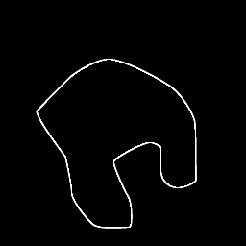
\includegraphics[width=5cm]{images/contour.png}~~~~~~~
  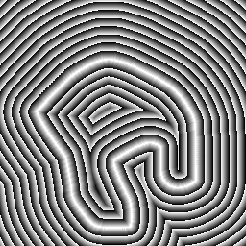
\includegraphics[width=5cm]{images/contour_circ.png} 
\end{center}


\begin{qu}
  Implement a function that digitizes an implicit shape (see
  MicroTutorial) on a digital grid with  step $h$.
\end{qu}

\begin{qu}
  Using a distance transformation on the shape and its complement,
  construct an implicit parametrization of the shape.
\end{qu}


\begin{qu}
  From this parametrization, implement  differential estimators such
  as normal vector field and curvature on surface point.
\end{qu}


\section{Multigrid Analysis}

\begin{qu}
  From this parametrization, implement  differential estimators such
  as normal vector field and curvature on boundary points. For
  example, you could consider finite difference analysis of the
  implicit function.
\end{qu}


\begin{qu}
  Perform a complete multigrid convergence evaluation with comparison
  to both expected quantities (available in \textsc{DGtal} for
  implicit shapes, cf  documentation) and estimated ones from other
  estimators (\emph{e.g.} estimators based on maximal DSS
  computations, cf documentation).
\end{qu}

\begin{qu}
  Please discuss about the quality of implicit parametrization based
  estimators (speed, quality...).
\end{qu}

\section{Extensions}


\begin{qu}
  Implement the same estimation on volumetric objects (\emph{i.e.} in
  $\mathbb{Z}^3$). For comparison, please consider normal vector and
  curvature estimators on digital surface implemented in \textsc{DGtal}.  
\end{qu}

\end{document}
